\documentclass[a4paper]{article}

%%% packages %%%%%%%%%%%%%%%%%%%%%%%%%%%%%%%%%%%%%%%%%%%%%%%%%%%%%%%%%%%%%%%%%
\usepackage{graphicx}
\usepackage{amsmath,amssymb}
\usepackage{alltt}
\usepackage{natbib} % please use \citep and \citet instead of \cite

\usepackage{hyperref}
\usepackage{xcolor}
\definecolor{dark-red}{rgb}{0.4,0.15,0.15}
\definecolor{dark-blue}{rgb}{0.15,0.15,0.8}
\definecolor{medium-blue}{rgb}{0,0,0.5}
\hypersetup{
	colorlinks, linkcolor={dark-red},
	citecolor={dark-blue}, urlcolor={medium-blue}
}

\graphicspath{{./figs/}}
\DeclareGraphicsExtensions{.pdf}

\setlength{\parindent}{0mm}

\usepackage{fancyhdr}

%%% %%%%%%%%%%%%%%%%%%%%%%%%%%%%%%%%%%%%%%%%%%%%%%%%%%%%%%%%%%%%%%%%%%%%%%%%%

\makeatletter
\newcommand{\seminar}{Seminar Cyber-Physical Systems (WS 2019/20)}
\title{\textbf{Prioritized Sweeping Neural DynaQ:\\ Boost Learning by Dreaming}}\let\Title\@title
\newcommand{\sTitle}{Prioritized Sweeping Neural DynaQ: Boost Learning by Dreaming}
\newcommand{\AuthorName}{Alexander Osiik}
\author{\AuthorName\\
	\href{mailto:alexander.osiik@student.uni-luebeck.de}{alexander.osiik@student.uni-luebeck.de}\\
	\small \seminar\\
%	\small Service Robotics Group\\
	\small Institute of Computer Engineering, University of L\"ubeck\\
}\let\Author\@author
\makeatother

\pagestyle{fancy}
\renewcommand{\footrulewidth}{0.4pt}
\lfoot{\seminar}
\cfoot{}
\rfoot{\thepage}
\lhead{\AuthorName}
\rhead{\sTitle}

%%% %%%%%%%%%%%%%%%%%%%%%%%%%%%%%%%%%%%%%%%%%%%%%%%%%%%%%%%%%%%%%%%%%%%%%%%%%

\begin{document}
	\maketitle
	
	\begin{abstract}
		\noindent%
		Hier beschreiben welche Hintergründe und Analogien aus der Biologie Reinforcement Learning hat.\\
		State of the Art.\\
		Was Zielsetzung im Original-Paper war, wie sie erreicht wurde und wie es im Projekt umgesetzt wurde.
	\end{abstract}
	
	
	\section{Introduction}
	\label{sec:introduction}
%	Swarm robotics~\citep{brambilla13} bla bla bla.
%	\citet{hamann18} describes bla bla bla
%	see Sec.~\ref{sec:results}
	\begin{itemize}
		\item Hier beschreiben welche Hintergründe und Analogien aus der Biologie Reinforcement Learning hat
		\item State of the Art, medizinische Aspekte, Forschungshintergründe
		\item Was Zielsetzung im Original-Paper, Übertragen der \textbf{hippocambal replays} auf RL.\\
		``... replay refers to the re-occurrence of a sequence of cell activations that also occurred during activity, but the replay has a much faster time scale.''
		\item Aufbau des Experiments
	\end{itemize}

	\section{Reinforcement Learning}
	\label{sec:rl}
	see Fig.~\ref{fig:image}	
	\begin{itemize}
		\item Einführung \textbf{Markov Decision Problem}
		\item Erklärung der Notation für \textit{state}, \textit{action}, \textit{transition function}, \textit{learning rate}, \textit{discount factor}
		\item Unterschiede \textit{value iteration}, \textit{policy extraction}, \textit{prioritized sweeping}
		\item spätestens hier müsste die Bellman Gleichung stehen:
		$$V^*(s) = \max_{a \in A} \sum_{s' \in S}^{} T(s,a,s')[R(s,a,s')+\gamma V^*(s')]$$
		\item Erklärung Q-Learning, Vorteile, Nachteile
		$$Q(s,a) \leftarrow Q(s,a) + \alpha[r + \gamma \max_{a' \in A}Q(s',a')-Q(s,a)]$$
		\item Exploration/Exploitation TradeOff und Techniken
		\item \textbf{HIER:} Idee des Papers: künstliche Erweiterung des State space umd RL für vergangenheitsabhängige Probleme anwendbar zu machen.
	\end{itemize}
	
	\section{GALMO}
	\label{sec:galmo}
	\begin{itemize}
		\item Vorstellung der Ergebnisse des Original Paper (GALMO)
	\end{itemize}
	
	\section{Project}
	\label{sec:project}
	\begin{itemize}
		\item Umsetzung von Q-Learning in Python
		\item DQN
		\item Implementierung GALMO?
	\end{itemize}
	
	\section{Results}
	\label{sec:results}
	
	
	\begin{figure}[t]
		\centering
		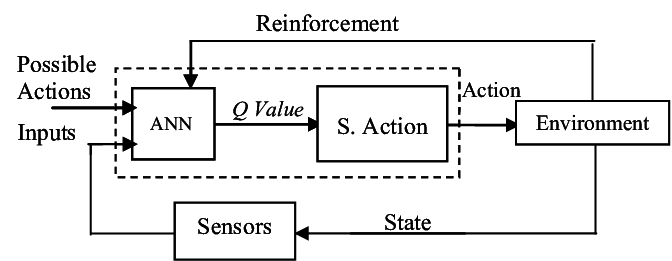
\includegraphics[angle=0,width=0.7\textwidth]{./figs/RL_ANN.png}
		\caption{\label{fig:image}Basic Q-Learning.}
	\end{figure}
	
	
	
	\section{Conclusion}
	
	
	\footnotesize
	\bibliographystyle{plainnat}
	\bibliography{./main}
	
\end{document}
